\section{Analysis of Results and Validation}

\subsection{Data Source and preproccesing: 16,301 Conversations with Elderly Users}

The initial stage of this research involved the curation of a large-scale conversational corpus. The raw data comprised approximately 30,561 sessions; however, to ensure the reliability of the self-disclosure analysis, a multi-stage preprocessing pipeline was applied to refine the dataset.

\begin{enumerate}
    \item \textbf{Filtering of Ludic Interactions:} Messages categorized under the \texttt{intent == games} label (e.g., riddles, word searches) were removed. These interactions are governed by rigid game logic rather than spontaneous social exchange, making them unsuitable for studying natural self-revelation.
    \item \textbf{System Message Cleaning:} Technical artifacts, such as the automated response \texttt{(pensando...)} generated during system latency, were purged. This ensures that the subsequent Natural Language Processing (NLP) tasks are performed strictly on human and intentional bot-generated content.
    \item \textbf{Minimal Interaction Constraint:} A threshold was set to exclude sessions with fewer than five total exchanges (human-bot turns). This criterion ensures that only sessions with enough conversational "mass" to exhibit depth are included in the study.
\end{enumerate}



As a result of this process, the final dataset was reduced to \textbf{16,301 valid sessions}. For data management purposes, each session was mapped from a composite identifier \newline \texttt{'\{user\_id\}\_\{session\_id\}.csv'}. This structured approach allows for efficient feature engineering while maintaining the integrity of the original conversational flows.


Beyond the total number of sessions, the dataset comprises \textbf{2,174 unique users}. The relationship between users and their respective number of interactions provides insight into the engagement patterns of the elderly population with the AI system.

\begin{figure}[htbp]
    \centering
    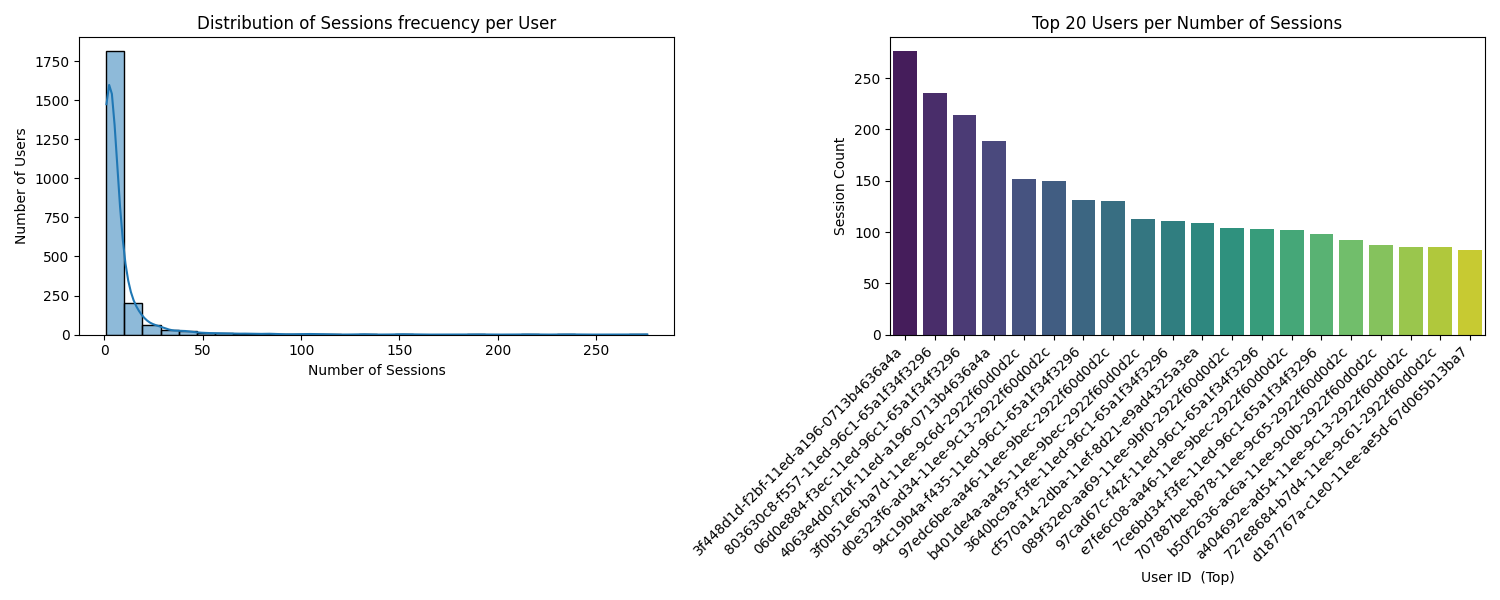
\includegraphics[width=0.8\textwidth]{images/user_dist.png}
    \caption{Distribution of the number of conversations per user (Top 20 most active users).}
    \label{fig:user_dist}
\end{figure}

As shown in Figure \ref{fig:user_dist}, there is a significant variance in user activity. This concentration of data in the most active users allows for a robust analysis of conversational depth, as these long-term interactions are more likely to transition from superficial "cliché" exchanges to more intimate layers of disclosure.

    \newpage
    \subsection{Programmatic Feature Engineering}

In addition to the semantic evaluation, a quantitative characterization of the sessions was performed through programmatic feature engineering. This process involved the extraction of objective metrics that describe the structural, temporal, and emotional dynamics of the human-computer interaction. While the semantic layers focus on \textit{what} is being said, these features provide crucial context on \textit{how} the interaction unfolds.

The engineered features can be categorized into three main groups:
\begin{itemize}
    \item \textbf{Structural and Temporal:} Metrics such as \texttt{session\_duration} and \texttt{n\_user\_interactions} quantify the level of engagement and the length of the conversational exchange.
    \item \textbf{Linguistic Complexity:} Features like \texttt{len\_user\_interactions} and \texttt{n\_proper\_nouns} serve as proxies for the richness of the discourse, where a higher density of proper nouns often correlates with the mention of specific personal entities or anecdotes.
    \item \textbf{Affective Analysis:} Sentiment scores (\texttt{pos}, \texttt{neu}, \texttt{neg}) were calculated for both the user and the bot. Comparing these allows for the assessment of emotional reciprocity, a key component in deepening social penetration.
\end{itemize}

\begin{table}[htbp]
\centering
\caption{Description of Programmatically Engineered Features.}
\label{tab:programmatic_features}
\begin{tabular}{@{}ll@{}}
\toprule
\textbf{Feature Name} & \textbf{Description}  \\ \midrule
\texttt{session\_duration} & Total duration of the session in seconds or minutes. \\
\texttt{n\_user\_interactions} & Total number of interactions initiated by the user. \\
\texttt{percentage\_user\_interactions} & User's share of interactions relative to the session total.  \\
\texttt{len\_user\_interactions} & Average length of the user's messages/inputs. \\
\texttt{n\_proper\_nouns} & Number of proper nouns detected in the conversation.\\
\texttt{user\_sent\_pos} & Positive sentiment score in the user's messages.\\
\texttt{user\_sent\_neu} & Neutral sentiment score in the user's messages. \\
\texttt{user\_sent\_neg} & Negative sentiment score in the user's messages. \\
\texttt{bot\_sent\_pos} & Positive sentiment score in the bot's responses. \\
\texttt{bot\_sent\_neu} & Neutral sentiment score in the bot's responses. \\
\texttt{bot\_sent\_neg} & Negative sentiment score in the bot's responses. \\ \bottomrule
\end{tabular}
\end{table}
    \subsection{Operationalizing Self-Disclosure Categories}

We have defined three primary categories that aggregate various conversational themes. These categories serve as proxies for the breadth and depth of the users' "social personality" layers:

\begin{itemize}
    \item \textbf{Category 1: Health and Well-being.} Focuses on the most immediate and vital concerns of the elderly population. It includes \textit{Mental and Emotional Health} as well as \textit{Physical Health and Addictions}.
    \item \textbf{Category 2: Interpersonal Relationships.} Maps the user's social circle and support system, encompassing \textit{Family Dynamics} and \textit{Affective/Romantic Relationships}.
    \item \textbf{Category 3: History and Personal Development.} Represents the deepest layers of the "onion," covering \textit{Personal Goals and Failures}, \textit{Traumas and Adversity}, and \textit{Professional Life and Career}.
\end{itemize}

\begin{table}[htbp]
\centering
\caption{Operationalized SPT Categories and Sub-themes.}
\label{tab:spt_categories}
\begin{tabular}{@{}ll@{}}
\toprule
\textbf{Main Category} & \textbf{Sub-themes / Dimensions} \\ \midrule
\textbf{C1: Health \& Well-being} & Mental Health, Emotional State, Physical Health, Addictions \\
\textbf{C2: Interpersonal Rel.} & Family Dynamics, Affective Relationships \\
\textbf{C3: Personal Development} & Goals \& Failures, Traumas \& Adversity, Career History \\ \bottomrule
\end{tabular}
\end{table}

This categorization allows the model to assign a numerical score to each session based on the presence and intensity of these topics, effectively creating a "disclosure profile" for every interaction.










\begin{figure}[htbp]
    \centering
    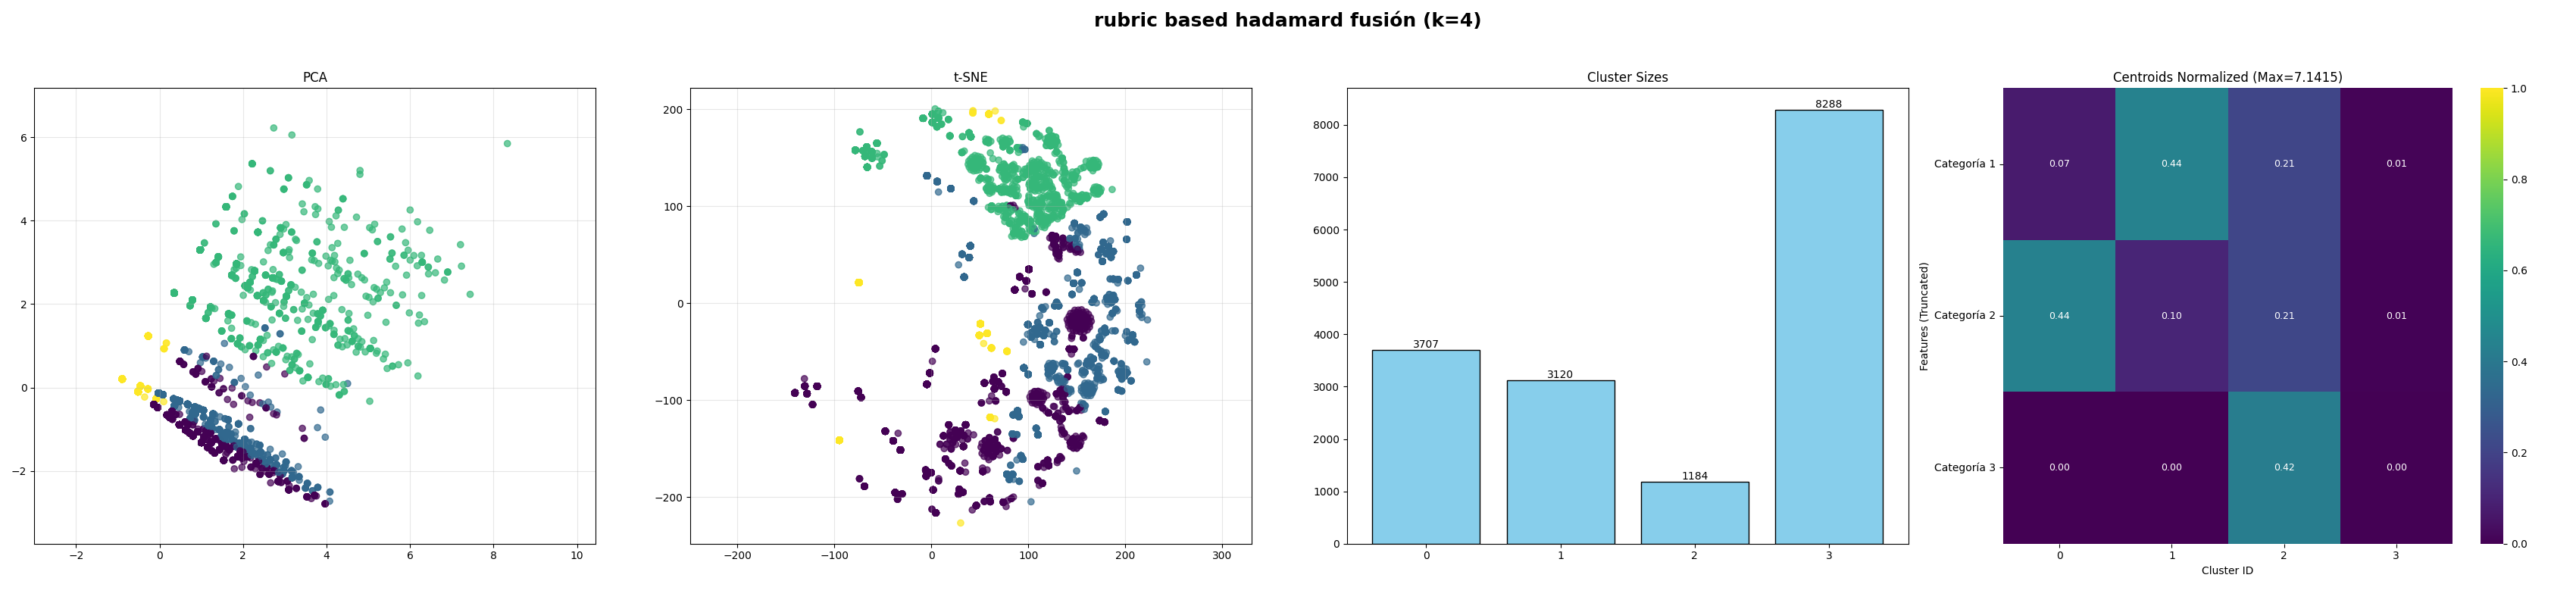
\includegraphics[width=\textwidth]{images/rubric_based_hadamard_fusion.png}
    \caption{Rubric Based Hadamard Fusion experiment.}
    \label{fig:rubric_based_hadamard}
\end{figure}

\begin{figure}[htbp]
    \centering
    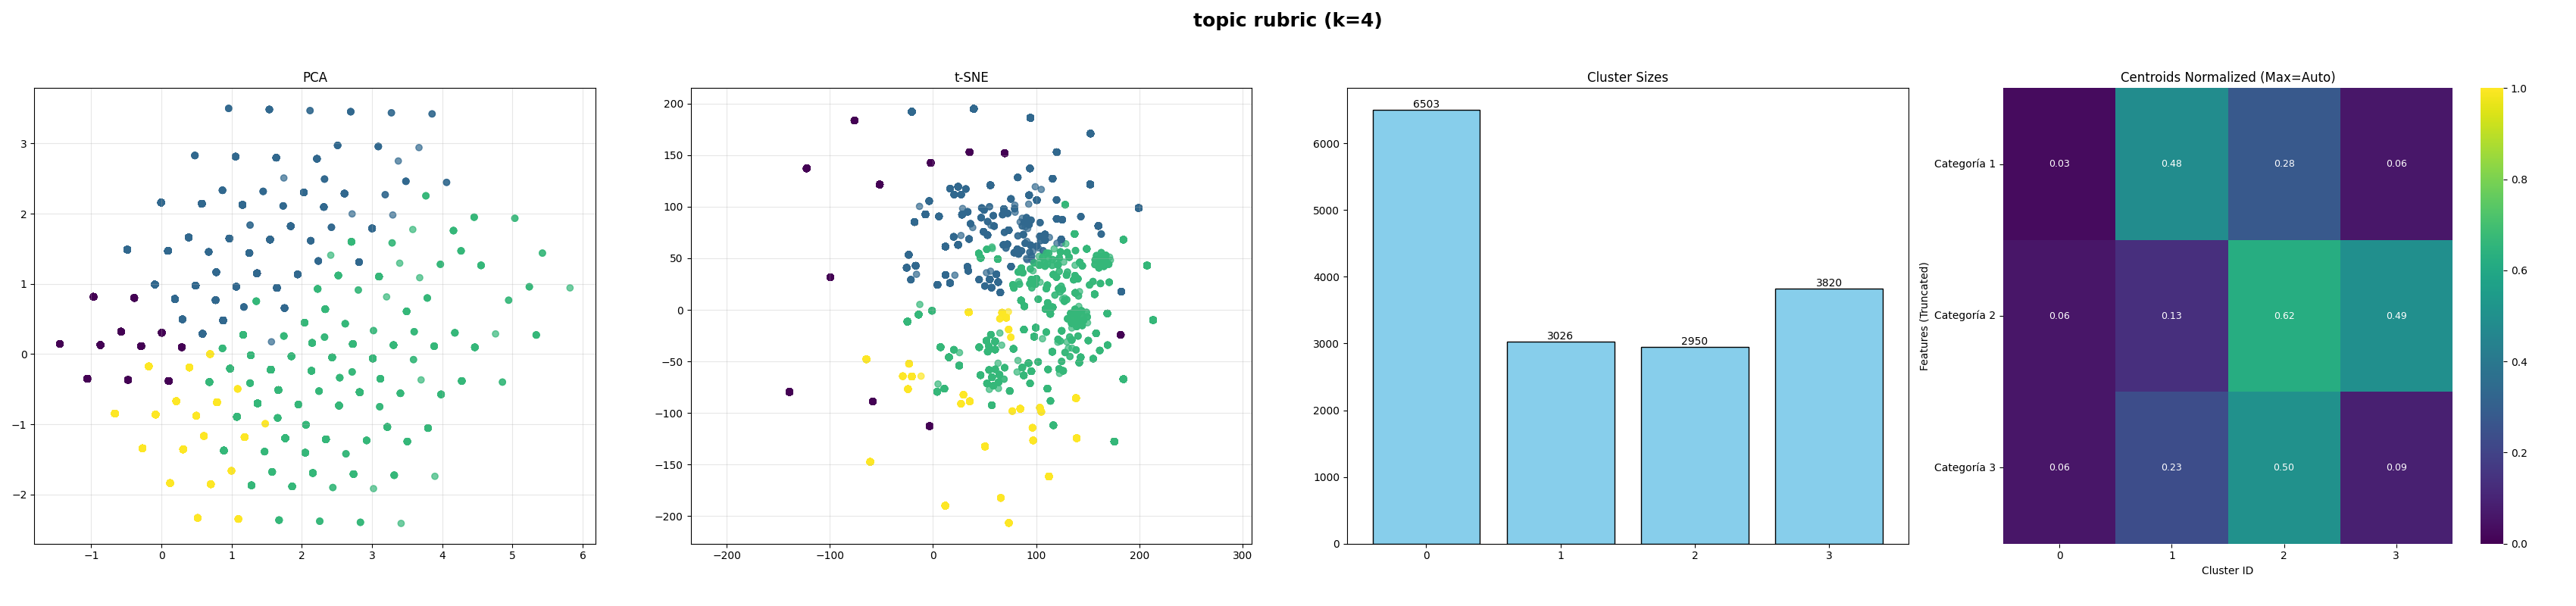
\includegraphics[width=\textwidth]{images/topic_rubric.png}
    \caption{Topic Rubric experiment.}
    \label{fig:topic_rubric}
\end{figure}

Comentar tamaños clusters, centroides, distribución espacial, etc
¿incluir los 6 experimentos?

   \subsection{Exploratory and Spacial Analysis}     
        
    %    \subsubsection{Cluster Characterization and Centroid Analysis}
    %    \subsubsection{Latent Space Visualization and Inter-Cluster Distances}

    \subsection{Experimental Evaluation}
        \subsubsection{Comparative Analysis of Feature Extraction Experiments}
        \subsubsection{Human-LLM Cross-Validation}


    \subsection{Fiability and Quality Standart}
        \subsubsection{Manual Labeling Protocol and Gold Standard Selection}

        contar como se han seleccionado las 130 sesiones. 
        
        \subsubsection{Inter-Rater Reliability: Krippendorff's Alpha Analysis}




    \subsection{Discussion of Unsuccessful Validation Metrics}

    \subsubsection{Full LLM Validation}
        Clústers -> sesiones más cercanas al centroide -> Caracterización con Gemini -> prompt gema descripción + sesion: categoría -> F1 \& MCC.
        Gráfica métricas en función distancia. 

    
    \subsection{Discussion: Discrepancy Analysis and LLM Bias}